\documentclass{article}

% 字体设置
\usepackage[no-math]{fontspec}
\setmainfont{Times New Roman}
\usepackage[UTF8]{ctex}
% \setCJKmainfont{Noto Serif SC}[ItalicFont=方正仿宋_GBK]
% \setCJKmathfont{Noto Serif SC}[ItalicFont=方正仿宋_GBK]

% 数学输入
\usepackage{amsmath}
\usepackage{amsfonts}
\usepackage{amssymb}
\usepackage{esint}
\usepackage{tikz}
\usepackage{latexsym}

% 排版设置
\usepackage{enumitem}
\usepackage{xcolor}
\usepackage{geometry}
% \geometry{a5paper}
% \geometry{left=0.3cm, right=0.3cm, top=1.7cm, bottom=1.7cm}
\geometry{a4paper}
\geometry{left=1.9cm, right=1.9cm, top=1.7cm, bottom=1.7cm}

% 表格
\usepackage{array}
\usepackage{tabularx}
\usepackage{caption}
\providecommand{\tightlist}{\setlength{\itemsep}{0pt}\setlength{\parskip}{0pt}}
\usepackage{siunitx}

% 超链接
\usepackage{hyperref}
\urlstyle{rm}
\hypersetup{
    colorlinks=true, 
    linkcolor=black, 
    citecolor=black, 
    urlcolor=black, 
    bookmarks=true, 
    bookmarksopen=true, 
    bookmarksnumbered=true, 
}

% 标题和作者设置
\title{实验 2 \quad 16 位比较器实验}
\author{Chen-Yuanmeng\thanks{Email: \url{chenyumeng23@mails.ucas.ac.cn}}}
\date{2024/10/31}

% 定义代码环境
\usepackage{listings}

\definecolor{codegreen}{rgb}{0, 0.6, 0}
\definecolor{codegray}{rgb}{0.5, 0.5, 0.5}
\definecolor{codepurple}{rgb}{0.58, 0, 0.82}
\definecolor{backcolour}{rgb}{0.95, 0.95, 0.92}

\definecolor{dkgreen}{rgb}{0,0.6,0}
\definecolor{gray}{rgb}{0.5,0.5,0.5}
\definecolor{mauve}{rgb}{0.58,0,0.82}
\lstset{
  frame=tb,
  aboveskip=3mm,
  belowskip=3mm,
  showstringspaces=false,
  columns=flexible,
  framerule=1pt,
  rulecolor=\color{gray!35},
  backgroundcolor=\color{gray!5},
  basicstyle={\small\ttfamily},
  numbers=none,
  numberstyle=\tiny\color{gray},
  keywordstyle=\color{blue},
  commentstyle=\color{dkgreen},
  stringstyle=\color{mauve},
  breaklines=true,
  breakatwhitespace=true,
  tabsize=3,
  language=Verilog
}

\begin{document}

\maketitle

\section{实验目的}

\begin{enumerate}\tightlist
    \item 熟悉 Verilog 编程、调试
    \item 熟悉简单比较器的工作原理
    \item 通过简单模块例化、连线实现复杂的数字电路
\end{enumerate}

\section{实验环境}

\begin{itemize}\tightlist
    \item Microsoft Windows 10.0.19045.5073
    \item Vivado v2017.4 (64-bit)
    \item 玉泉路一机房
\end{itemize}

\section{原理说明}

\subsection{16位比较器}

16位比较器由4个4位比较器相连而成. 一个4位比较器有高位输入, 本位数字输入两种输入, 输出为大于/等于/小于三种可能. 具体情况如下:
\begin{enumerate}\tightlist
    \item 当高位输入为 ``>'' 时, 输出为 ``>'';
    \item 当高位输入为 ``='' 时: \begin{enumerate}\tightlist
        \item 当本位数字 \(A > B\) 时, 输出为 ``>'';
        \item 当本位数字 \(A = B\) 时, 输出为 ``='';
        \item 当本位数字 \(A < B\) 时, 输出为 ``<''.
    \end{enumerate}
    \item 当高位输入为 ``<'' 时, 输出为 ``<''.
\end{enumerate}

要将4位比较器扩展到16位比较器, 则需要先比较16位数字中的最高4位, 再依次比较更低位. 故, 高位的输出应与低位的输入部分相连, 最高位输入应为 ``='', 最低位输出即为16位比较器的输出.

在实际设计过程中, 我们需要在 \lstinline|comp_16| 模块中\textbf{例化} 4个 \lstinline|comp_4| 模块的示例, 进行对其的调用. 这是模块化设计思想的体现, 可以让代码复用减少, 增加程序的可读性和易维护性.

\subsection{4位超前进位加法器}

超前进位加法器相比串行加法器, 可以实现更快速的计算. 其原理是, 加到第 \(i\) 位的进位输入信号是两个加数第 \(i\) 位以前各位的函数,可在相加前由 \(A\), \(B\) 两数确定.

设 \(G_i=A_iB_i\) 为进位生成函数, \(P_i=A_i + B_i\) 为进位传递函数. 此时可以得到 \begin{align*}
    (CO)_i & = G_i + P_i (CI)_i \\
    & = G_i + P_i (G_{i-1} + P_{i-1} (CI)_{i-1}) \\
    & = G_i + P_i G_{i-1} + P_i P_{i-1} (G_{i-2} + P_{i-2} (CI)_{i-2}) \\
    & = \cdots \\
    & = G_i + P_i G_{i-1} + P_i P_{i-1} G_{i-2} + \cdots + P_i P_{i-1} \cdots P_1 G_0 + P_i P_{i-1} \cdots P_1 P_0 (CI)_0,
\end{align*} 而 \[S_i = A_i \oplus B_i \oplus (CI)_i.\]

据此即可得到每一位的进位输入, 进而进行超前进位.

\section{接口定义}

\subsection{4位比较器}

4位比较器的接口定义如下:
\begin{lstlisting}
    module comp_4(
        input [3:0] A,          // 输入的待比较数字 A
        input [3:0] B,          // 输入的待比较数字 B
        input in_A_G_B,         // 高位输入, 表示高位A>B
        input in_A_E_B,         // 高位输入, 表示高位A=B或没有数字
        input in_A_L_B,         // 高位输入, 表示高位A<B
        output out_A_G_B,       // 输出, 为1时表示 A>B
        output out_A_E_B,       // 输出, 为1时表示 A=B
        output out_A_L_B        // 输出, 为1时表示 A<B
    );
\end{lstlisting}


\subsection{16位比较器}

16位比较器的接口定义如下:
\begin{lstlisting}
    module comp_16(
        input [15:0] A,         // 输入的待比较数字 A
        input [15:0] B,         // 输入的待比较数字 A
        output out_A_G_B,       // 输出, 为1时表示 A>B
        output out_A_E_B,       // 输出, 为1时表示 A=B
        output out_A_L_B        // 输出, 为1时表示 A<B
    );
\end{lstlisting}

\subsection{4位超前进位加法器}

16位比较器的接口定义如下:
\begin{lstlisting}
    module cla_adder_4(
        input [3:0] A,          // 加数 A
        input [3:0] B,          // 加数 B
        input Cin,              // 输入进位
        output [3:0] S,         // 输出位
        output Cout             // 输出进位
    );
\end{lstlisting}


\section{调试过程及结果}

点击左侧 ``SIMULATION'' 下的 ``Run Simulation'', 以默认设置进行模拟调试. 调试结果分别如图所示:

\subsection{4位比较器}

\begin{center}
    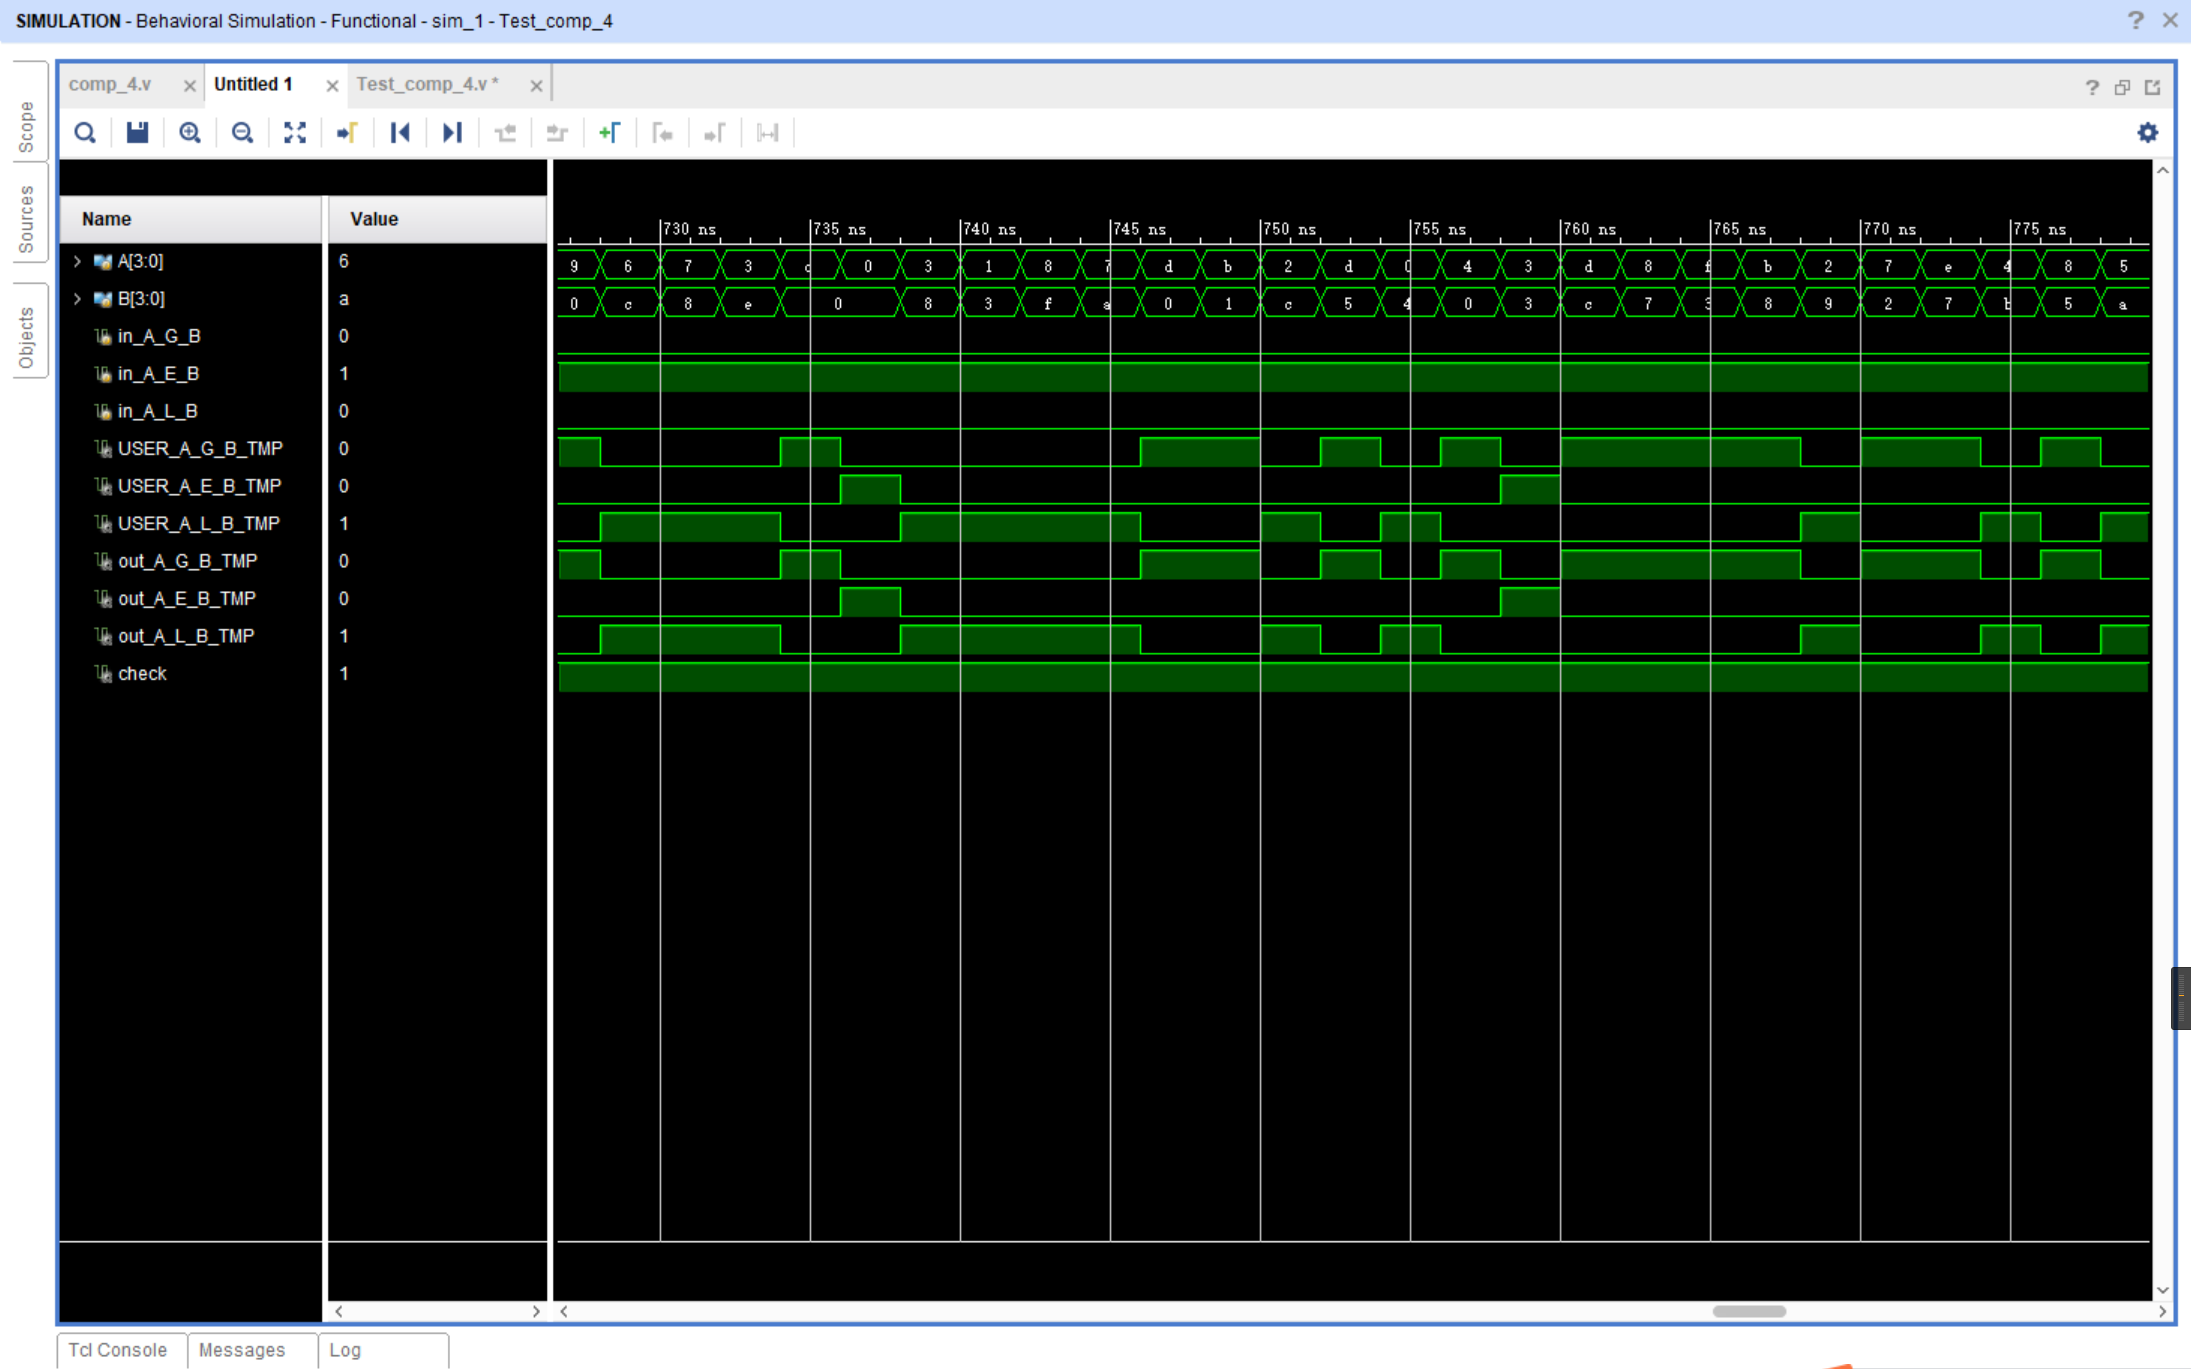
\includegraphics[width=500pt]{assets/image_comp_4.png}
    \captionof{figure}{4位比较器 Simulation 结果}
\end{center}

\subsection{16位比较器}

\begin{center}
    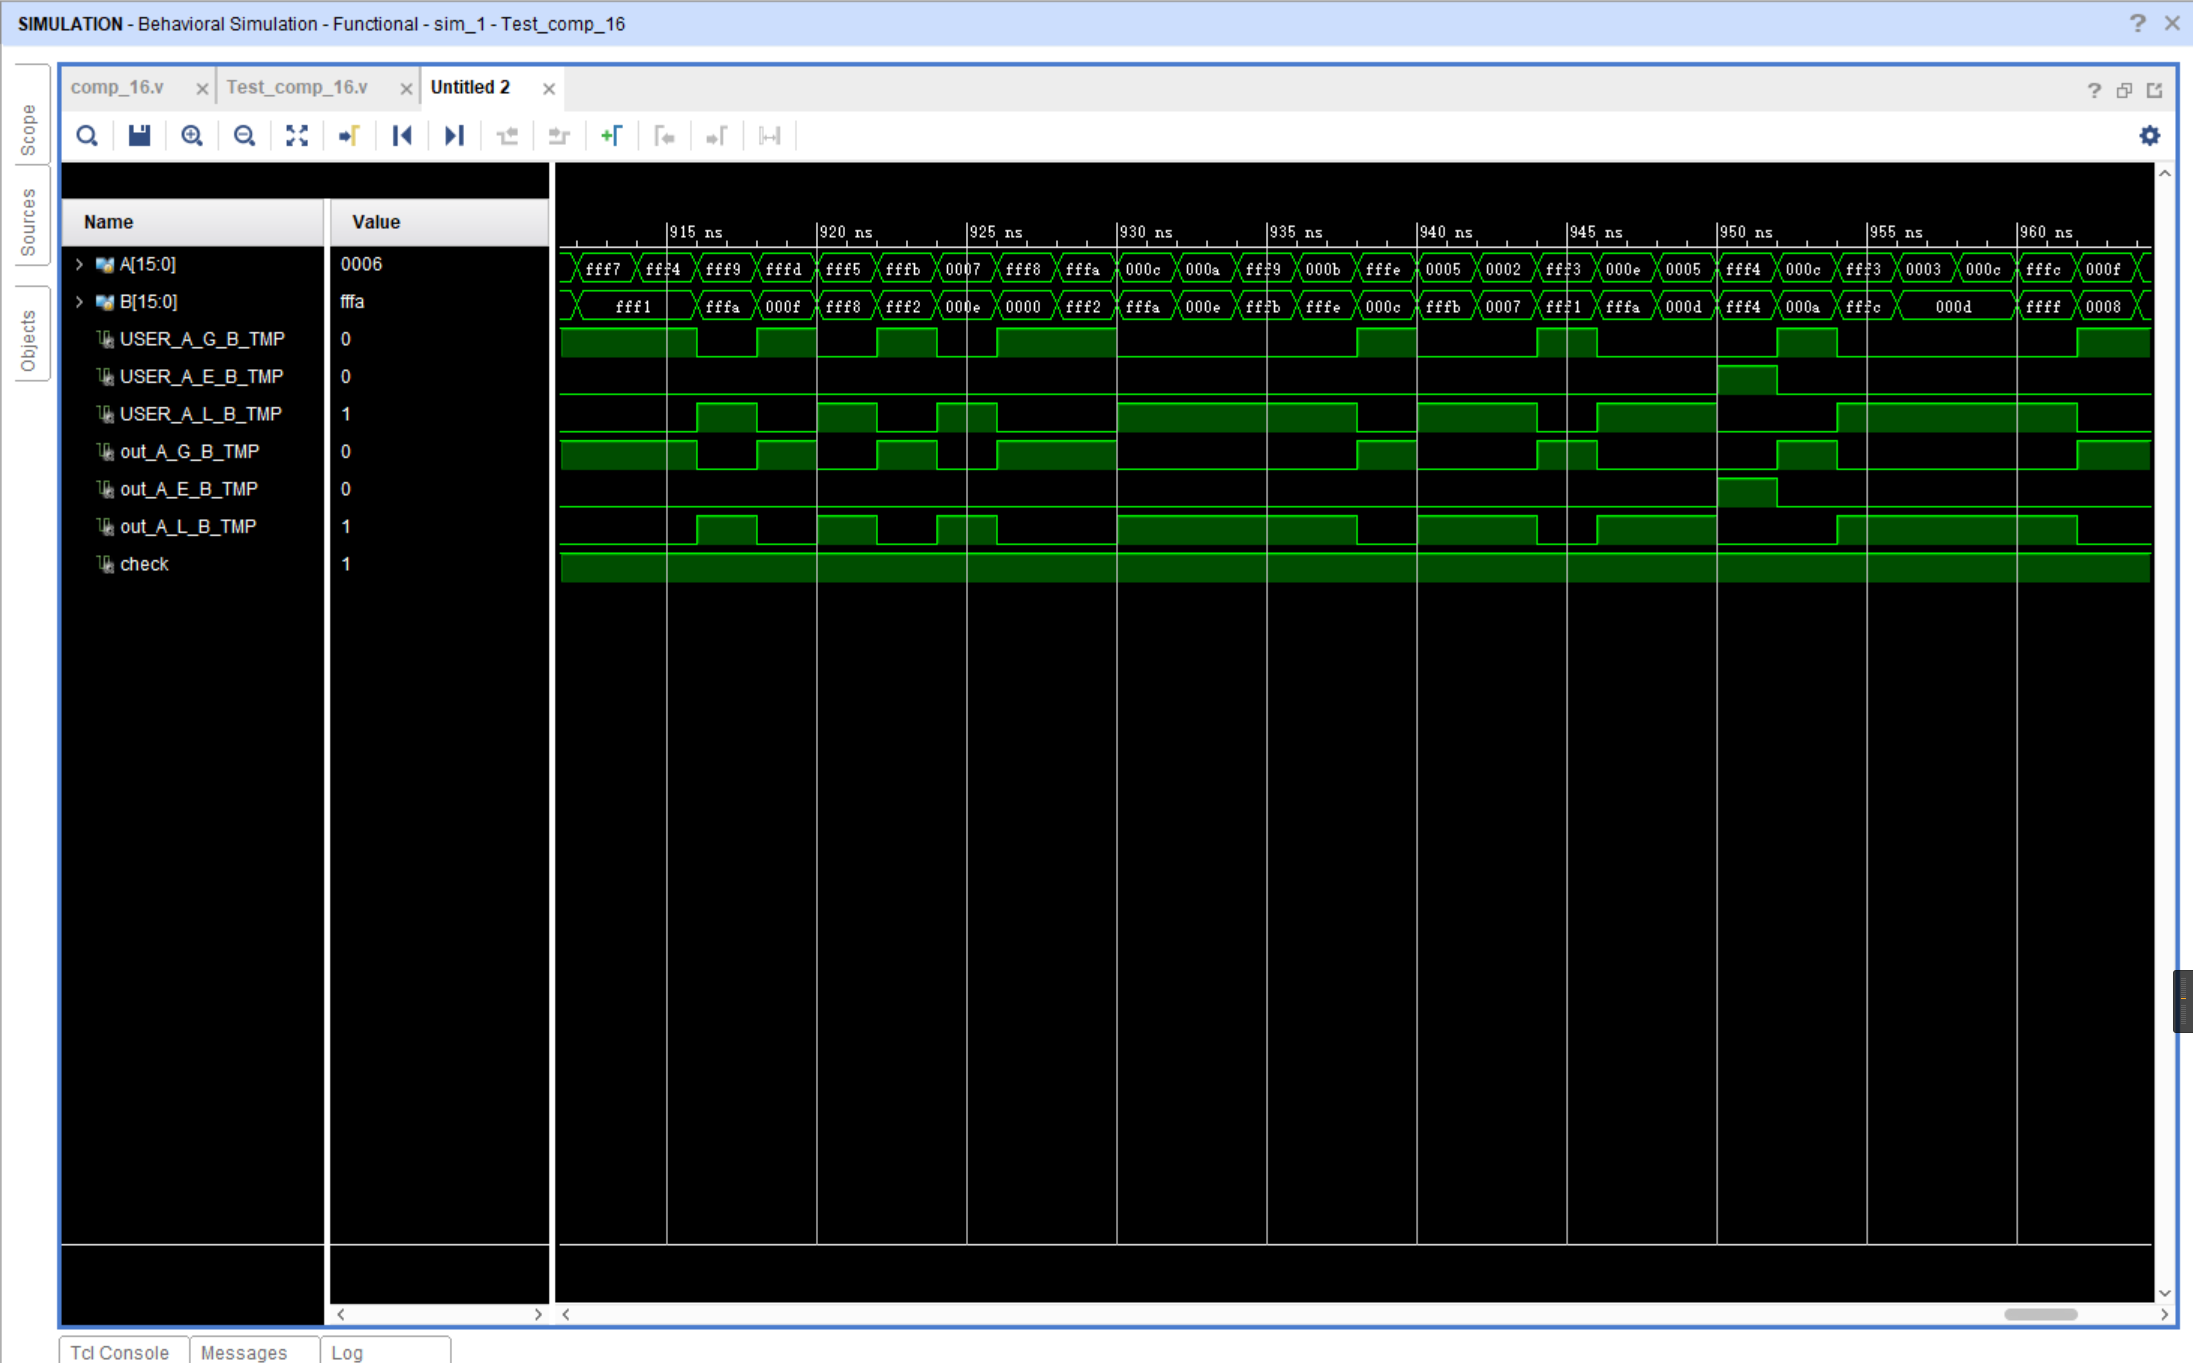
\includegraphics[width=500pt]{assets/image_comp_16.png}
    \captionof{figure}{全加器 Simulation 结果}
\end{center}

\subsection{4位超前进位加法器}

\begin{center}
    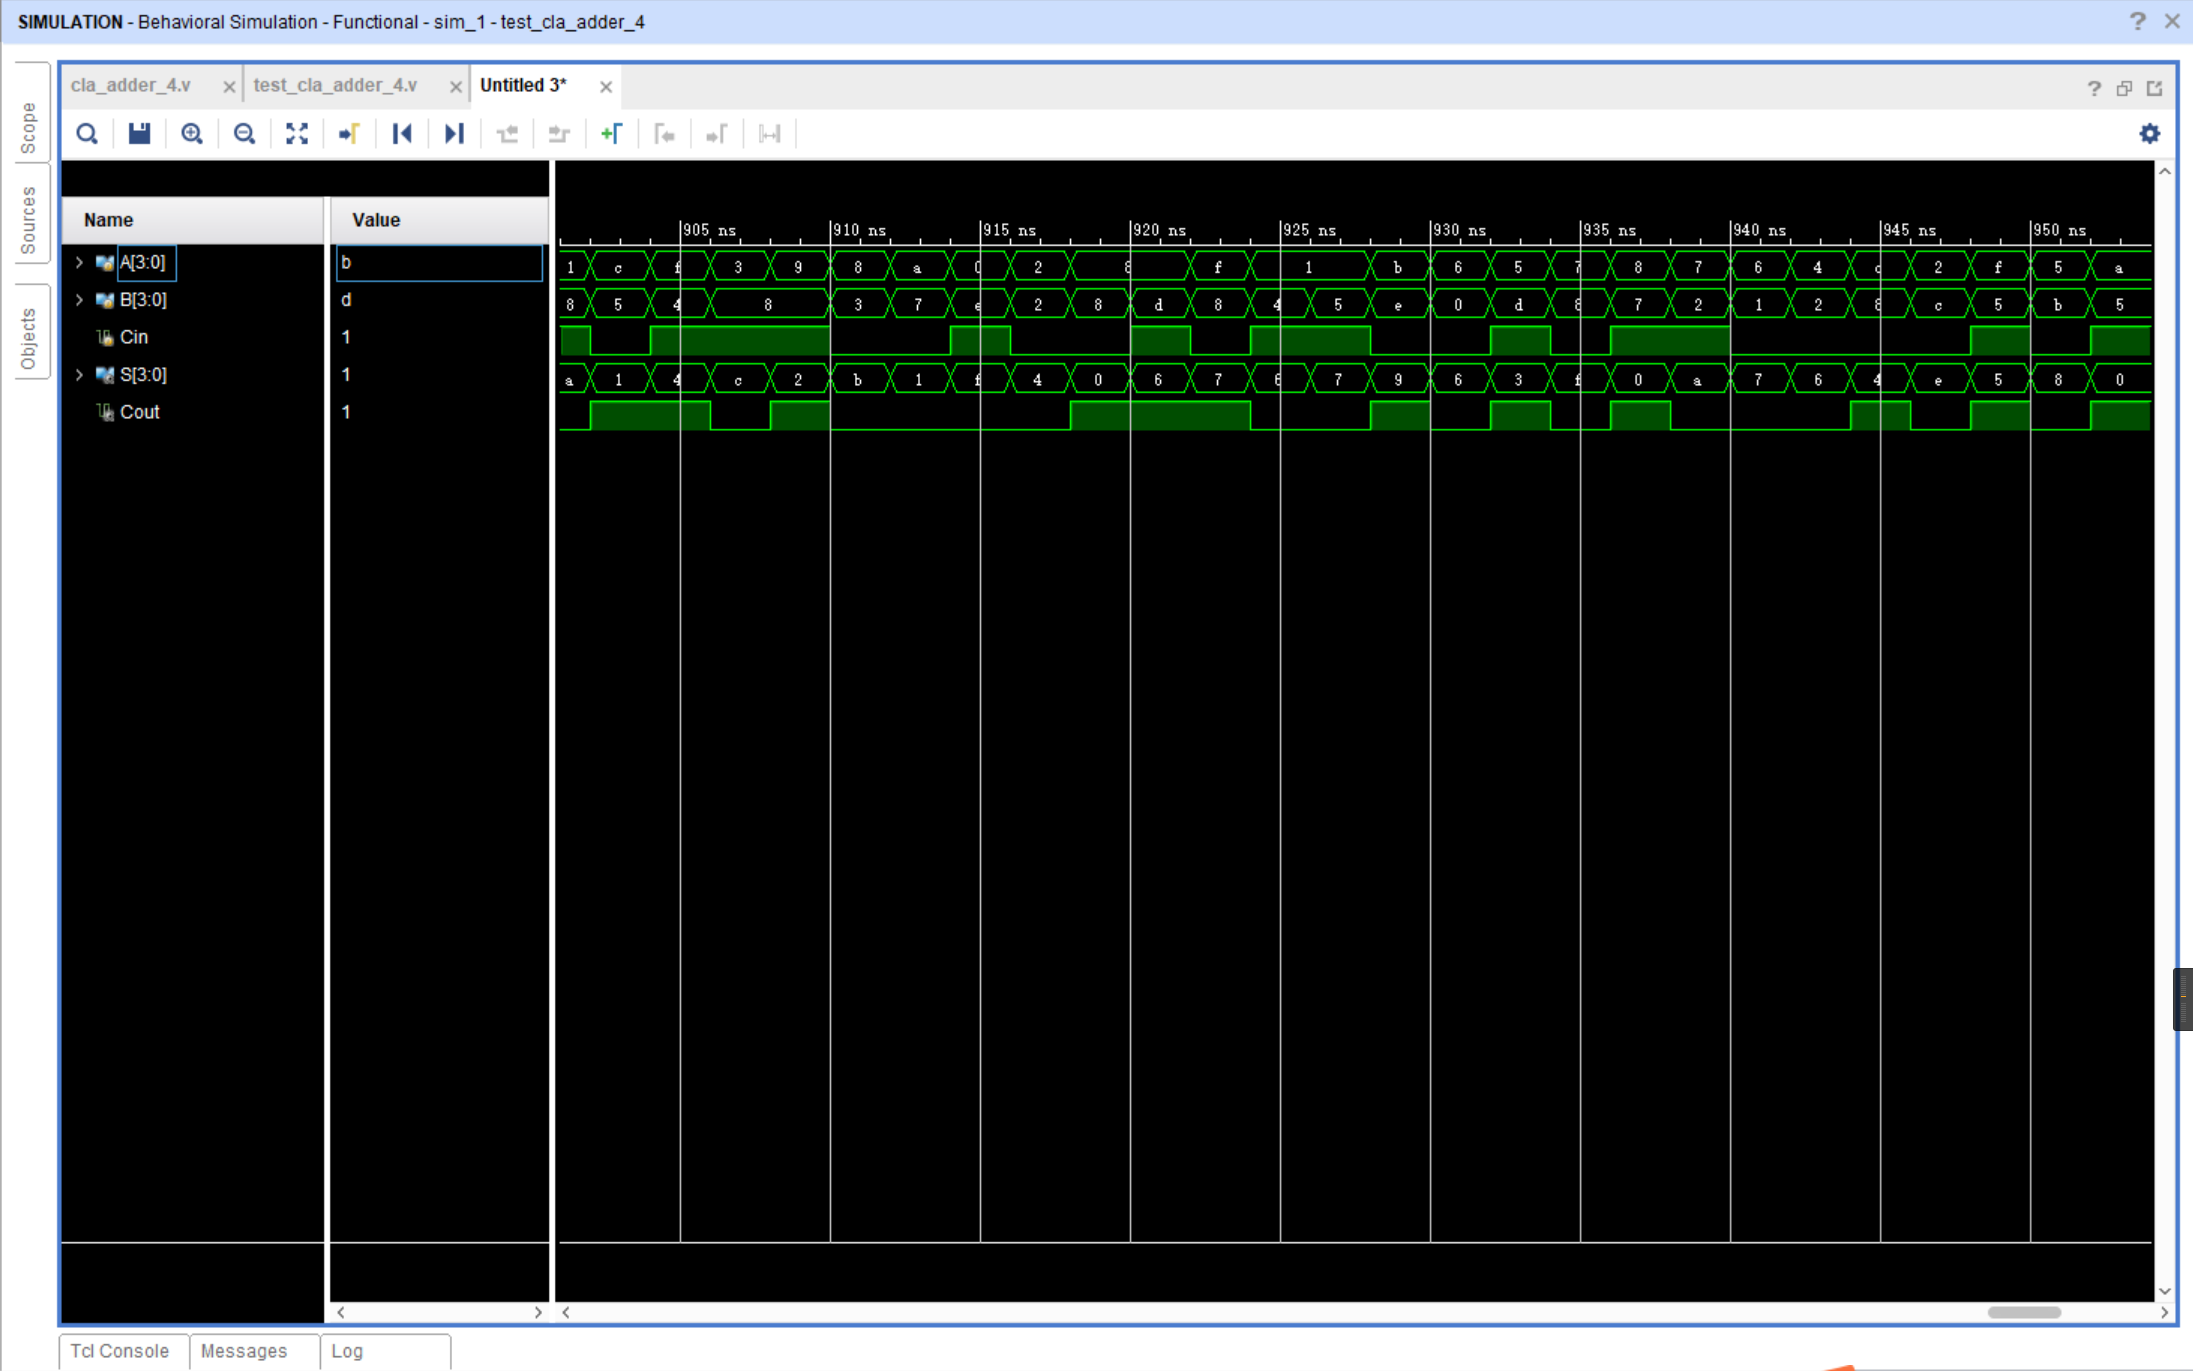
\includegraphics[width=500pt]{assets/image_cla_adder_4.png}
    \captionof{figure}{3--8译码器 Simulation 结果}
\end{center}

\section{实验总结}

通过本次实验, 我了解并实践了 Vivado 模块化设计的思想, 并对比较器和超前进位加法器的结构有了更深刻的认识. 此外, 我纠正了对于 \lstinline|always| 语句的错误认识, 对组合逻辑电路和时序逻辑电路在 Verilog 设计中的不同有了更深刻的了解.


\section{源代码}

\subsection{16位比较器}

\subsubsection{4位比较器}

File: comp\_4.v
\begin{lstlisting}
    `timescale 1ns / 1ps

    module comp_4(
        input [3:0] A,
        input [3:0] B,
        input in_A_G_B,
        input in_A_E_B,
        input in_A_L_B,
        output out_A_G_B,
        output out_A_E_B,
        output out_A_L_B
        );
        
        reg A_G_B, A_E_B, A_L_B;
        
        always @(*) begin
        if (in_A_G_B == 1 && in_A_E_B == 0 && in_A_L_B == 0) begin
            A_G_B = 1;
            A_E_B = 0;
            A_L_B = 0;
            end
        else if (in_A_G_B == 0 && in_A_E_B == 1 && in_A_L_B == 0) begin
            A_G_B = 0;
            A_E_B = 0;
            A_L_B = 0;
            if (A>B)
                A_G_B = 1;
            else if (A == B)
                A_E_B = 1;
            else
                A_L_B = 1;
            end
        else begin
            A_G_B = 0;
            A_E_B = 0;
            A_L_B = 1;
            end
        end
        
        assign out_A_G_B = A_G_B;
        assign out_A_E_B = A_E_B;
        assign out_A_L_B = A_L_B;
          
    endmodule    
\end{lstlisting}

File: test\_comp\_4.v
\begin{lstlisting}
    `timescale 1ns / 1ps

    module Test_comp_4(
    
        );
    
    // ports you get
    reg [3:0] A;
    reg [3:0] B;
    reg in_A_G_B;
    reg in_A_E_B;
    reg in_A_L_B;
    wire USER_A_G_B_TMP;
    wire USER_A_E_B_TMP;
    wire USER_A_L_B_TMP;
    
    // ports you needn't care at writing
    wire out_A_G_B_TMP;
    wire out_A_E_B_TMP;
    wire out_A_L_B_TMP;
    wire check = (USER_A_G_B_TMP === out_A_G_B_TMP) && (USER_A_E_B_TMP === out_A_E_B_TMP) && (USER_A_L_B_TMP === out_A_L_B_TMP); 
    
    TEMPLATE_COMP_4 inst_comp_4_0 (
        .A(A),
        .B(B),
        .in_A_G_B(in_A_G_B),
        .in_A_E_B(in_A_E_B),
        .in_A_L_B(in_A_L_B),
        .out_A_G_B(out_A_G_B_TMP),
        .out_A_E_B(out_A_E_B_TMP),
        .out_A_L_B(out_A_L_B_TMP)
        );
    
    // instantiate your module
    /****************************** WRITE YOUR CODE HERE ********************************/
    comp_4 inst_comp_4(
        .A(A),
        .B(B),
        .in_A_G_B(in_A_G_B),
        .in_A_E_B(in_A_E_B),
        .in_A_L_B(in_A_L_B),
        .out_A_G_B(USER_A_G_B_TMP),
        .out_A_E_B(USER_A_E_B_TMP),
        .out_A_L_B(USER_A_L_B_TMP)
    );
    /****************************** WRITE YOUR CODE HERE ********************************/
    
    initial begin
        A = 4'd1;
        B = 4'd0;
        in_A_G_B=1'b0;
        in_A_E_B=1'b1;
        in_A_L_B=1'b0;
    end
    
    always  begin
        #2;
        A = $random() % 16;
        B = $random() % 16;
    end
    
    endmodule    
\end{lstlisting}

\subsubsection{16位比较器}

File: comp\_4.v
\textbf{同上 \texttt{comp\_4.v}.}

File: comp\_16.v
\begin{lstlisting}
    `timescale 1ns / 1ps

    module comp_16(
        input [15:0] A,
        input [15:0] B,
        output out_A_G_B,
        output out_A_E_B,
        output out_A_L_B
        );
    
        wire mid_A_G_B_1, mid_A_E_B_1, mid_A_L_B_1;
        wire mid_A_G_B_2, mid_A_E_B_2, mid_A_L_B_2;
        wire mid_A_G_B_3, mid_A_E_B_3, mid_A_L_B_3;
    
        comp_4 comp_4_1 (
            .A(A[15:12]),
            .B(B[15:12]),
            .in_A_G_B(1'b0),
            .in_A_E_B(1'b1),
            .in_A_L_B(1'b0),
            .out_A_G_B(mid_A_G_B_1),
            .out_A_E_B(mid_A_E_B_1),
            .out_A_L_B(mid_A_L_B_1)
        );
    
        comp_4 comp_4_2 (
            .A(A[11:8]),
            .B(B[11:8]),
            .in_A_G_B(mid_A_G_B_1),
            .in_A_E_B(mid_A_E_B_1),
            .in_A_L_B(mid_A_L_B_1),
            .out_A_G_B(mid_A_G_B_2),
            .out_A_E_B(mid_A_E_B_2),
            .out_A_L_B(mid_A_L_B_2)
        );
    
        comp_4 comp_4_3 (
            .A(A[7:4]),
            .B(B[7:4]),
            .in_A_G_B(mid_A_G_B_2),
            .in_A_E_B(mid_A_E_B_2),
            .in_A_L_B(mid_A_L_B_2),
            .out_A_G_B(mid_A_G_B_3),
            .out_A_E_B(mid_A_E_B_3),
            .out_A_L_B(mid_A_L_B_3)
        );
    
        comp_4 comp_4_4 (
            .A(A[3:0]),
            .B(B[3:0]),
            .in_A_G_B(mid_A_G_B_3),
            .in_A_E_B(mid_A_E_B_3),
            .in_A_L_B(mid_A_L_B_3),
            .out_A_G_B(out_A_G_B),
            .out_A_E_B(out_A_E_B),
            .out_A_L_B(out_A_L_B)
        );
    
    endmodule
\end{lstlisting}

File: test\_comp\_16.v
\begin{lstlisting}
    `timescale 1ns / 1ps

    module Test_comp_16(
    
        );
    
        // ports you get
        reg [15:0] A;
        reg [15:0] B;
        wire USER_A_G_B_TMP;
        wire USER_A_E_B_TMP;
        wire USER_A_L_B_TMP;
    
        // ports you needn't care at writing
        wire out_A_G_B_TMP;
        wire out_A_E_B_TMP;
        wire out_A_L_B_TMP;
        wire check = (USER_A_G_B_TMP === out_A_G_B_TMP) && (USER_A_E_B_TMP === out_A_E_B_TMP) && (USER_A_L_B_TMP === out_A_L_B_TMP);
    
        TEMPLATE_COMP_16 inst_comp_16_0 (
        .A(A),
        .B(B),
        .A_G_B(out_A_G_B_TMP),
        .A_E_B(out_A_E_B_TMP),
        .A_L_B(out_A_L_B_TMP)
        );
        
        // instantiate your module
        /****************************** WRITE YOUR CODE HERE ********************************/
        comp_16 inst_comp_16 (
        .A(A),
        .B(B),
        .out_A_G_B(USER_A_G_B_TMP),
        .out_A_E_B(USER_A_E_B_TMP),
        .out_A_L_B(USER_A_L_B_TMP)
        );
        /****************************** WRITE YOUR CODE HERE ********************************/
    
        initial begin
            A = 16'd1;
            B = 16'd0;
        end
    
        always  begin
            #2;
            A = $random() % 16;
            B = $random() % 16;
        end
    
    endmodule    
\end{lstlisting}

\subsection{4位超前进位加法器}

File: cla\_adder\_4.v
\begin{lstlisting}
    `timescale 1ns / 1ps

    module cla_adder_4(
        input [3:0] A,
        input [3:0] B,
        input Cin,
        output [3:0] S,
        output Cout
        );
    
        wire [3:0] G;
        wire [3:0] P;
        wire [3:0] C;
    
        assign G = A & B;
        assign P = A ^ B;
    
        assign C[0] = G[0] | (P[0] & Cin);
        assign C[1] = G[1] | (P[1] & G[0]) | (P[1] & P[0] & Cin);
        assign C[2] = G[2] | (P[2] & G[1]) | (P[2] & P[1] & P[0] & Cin);
        assign C[3] = G[3] | (P[3] & G[2]) | (P[3] & P[2] & P[1] & P[0] & Cin);
    
        assign S = A ^ B ^ {C[2:0], Cin};
    
        assign Cout = C[3];
    endmodule    
\end{lstlisting}

File: test\_cla\_adder\_4.v
\begin{lstlisting}
    `timescale 1ns / 1ps

    module test_cla_adder_4();
    
        reg [3:0] A, B;
        reg Cin;
        wire Cout;
        wire [3:0] S;
    
        cla_adder_4 inst_cla_add_4 (
            .A(A),
            .B(B),
            .Cin(Cin),
            .S(S),
            .Cout(Cout)
        );
    
        initial begin
        A = 1'b0;
        B = 1'b0;
        Cin = 1'b0;
        end
    
        always begin
        #2;
        A = $random() % 16;
        B = $random() % 16;
        Cin = $random() % 2;
        end
    
    endmodule    
\end{lstlisting}

\end{document}